\documentclass[a1,portrait]{a0poster}
\usepackage[brazil]{babel}
\usepackage[utf8]{inputenc}
\usepackage[absolute]{textpos} 
\usepackage{graphicx}
\usepackage{color}
\usepackage{xcolor}
\usepackage{amsmath,amssymb}
\usepackage{booktabs}

\definecolor{DarkBlue}{rgb}{0.1,0.1,0.5}
\definecolor{Red}{rgb}{0.9,0.0,0.1}
\definecolor{DarkGreen}{rgb}{0.10,0.50,0.10}

\let\Textsize\normalsize
\def\Head#1{\noindent\hbox to \hsize{\hfil{\LARGE\color{DarkBlue} #1}}\bigskip}
\def\LHead#1{\noindent{\LARGE\color{DarkBlue} #1}\smallskip}
\def\Subhead#1{\noindent{\large\color{DarkBlue} #1}}
\newcommand{\quiteHuge}{\fontsize{55}{70}\selectfont}
\def\Title#1{\begin{center}\noindent{\quiteHuge\color{DarkGreen}#1}\end{center}}

\TPGrid[40mm,40mm]{23}{12}

\parindent=0pt
\parskip=0.5\baselineskip

\begin{document}

\begin{figure}[h]
\centering

\includegraphics[width=18cm]{unb-extenso.jpg}
\end{figure}

\begin{textblock}{23}(0,0)
\vspace{0.5cm}
\Title{\textsc{Gestão do Gêmeo Digital de Reciclagem em Cooperativas sob a Ótica da Privacidade (SIPA)}}
\end{textblock}

\begin{textblock}{23}(0,0.65)
    \begin{center}
        \parbox{0.8\textwidth}{
            \small
    \begin{center}
    \textbf{Autores -- Grupo Reciclagem 1}\\
    \begin{tabular}{@{}l@{\hspace{0.5cm}}r@{\hspace{1.5cm}}r@{\hspace{0.5cm}}l@{}}
    Filipe Alves de Sousa & 261108383 & 262114213 & Emanuel Brandão de Galvão Correia\\
    Ruben Isaac Dias da Silva & 262115391 & 261107680 & Carlos Eduardo da Silva Papa
    \end{tabular}\\
    \textbf{Disciplina:} Gestão de Projetos de TI (GPTI) -- PPCA/CIC/UnB\\
    \textbf{Componente:} \texttt{SRSR3.SIPA-CC} / \texttt{DSRSR3.SIPA-CC} | \textbf{Código:} 3p2 / 3R31
    \end{center}
}
\end{center}
\end{textblock}

\begin{textblock}{11}(0,1.65)

\LHead{1. Introdução e Paradigma Digital Twin-First}

Este projeto propõem a modelagem de governança para a planta de reciclagem de plásticos ($R3$) operada por cooperativas no DF. Adotando o PMBOK 8ª Edição estendido pela estrutura \texttt{GPH.SIPA}, o Gêmeo Digital ($DSR$) deixa de ser mera réplica passiva e passa a atuar como Referência de Decisão (\emph{Decision Reference}), orientando a evolução do sistema real ($RSR$).

\vspace{0.3cm}
\LHead{2. Modelagem Tetraédrica F/S/P/C}

A caracterização do sistema utiliza a abordagem sistêmica de Gharajedaghi (2011), integrando Função, Estrutura, Processo e Contexto com foco em Privacidade (LGPD).

\vspace{0.25cm}
\begin{figure}[h!]
\centering
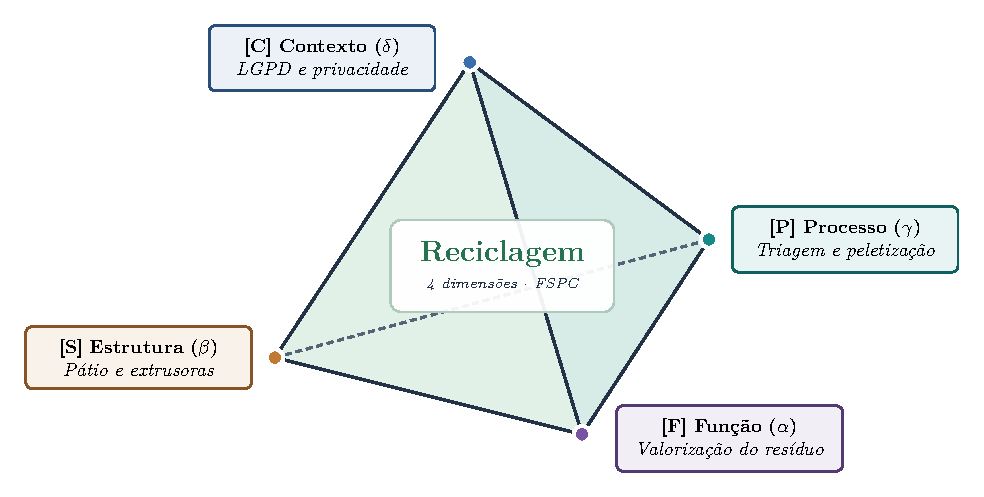
\includegraphics[width=25cm]{out/tetra1.pdf}
\caption{Estrutura Tetraédrica $F/S/P/C$ Integrada.}
\end{figure}

\vspace{0.3cm}
\LHead{3. Pesquisa Bibliométrica (Web of Science)}

Realizou-se o afunilamento bibliométrico na base Web of Science (CAPES/CAFe) para isolar a literatura de interseção entre reciclagem, Gêmeos Digitais e Privacidade:
\begin{itemize}\raggedright
    \item \textbf{Busca Base ($R3$):} \texttt{TS=("solid* wast* rec*")} -- 59.765 docs.
    \item \textbf{Volume Sintético (4D):} \texttt{TS=(func* AND struct*}\allowbreak\texttt{ AND proc* AND cont*)} -- 14 docs.
    \item \textbf{Afunilamento Grupo (3p2):} \texttt{TS=(("solid* wast* rec*") AND}\allowbreak\texttt{ ("digital twin" OR "IoT") AND}\allowbreak\texttt{ ("privacy" OR "LGPD"))}.
    
    \item \textbf{Reciclagem:} \texttt{(((TS=(recycl* OR "material recover*" OR "resource recover*" OR valoriz* OR valoris*)) AND (TS=("digital twin*"))) AND (TS=(disassembl* OR dismantl* OR demanufactur* OR "waste sort*" OR "reverse logistic*"))) NOT (TS=("solid waste*" OR "municipal waste*" OR "urban waste*" OR "post-consumer waste*" OR "electronic waste*" OR "e-waste"))}

    \item \textbf{Privacidade:} \texttt{(TS=("digital twin*")) AND (TS=(LGPD OR GDPR OR "Lei Geral de Proteção de Dados" OR "General Data Protection Regulation" OR "Brazilian General Data Protection Law" OR "privacy regulat*" OR "data protection law*"))}
\end{itemize}

\end{textblock}

\begin{textblock}{11}(12,1.65)

\LHead{4. Arquitetura de Capacidades DTC e Agentes de IA}

Mapeamento entre o O QUÊ (DTC/CPT) e o COMO (DTC/AIACPT) para a especificação dos Agentes de IA (A1 Conversacional, A2 Workflow LGPD, A3 Autônomo e A4 MAGS Multiagentes).

\vspace{0.25cm}
\begin{figure}[h!]
\centering
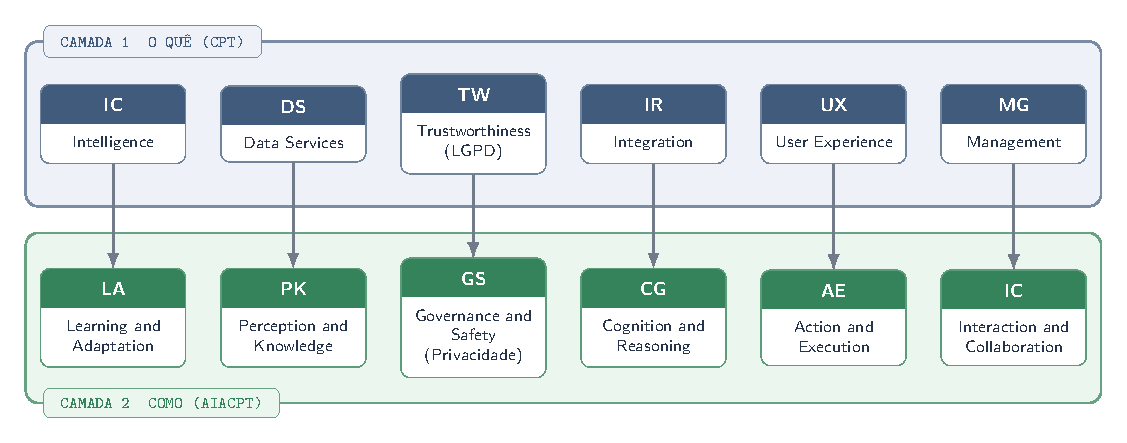
\includegraphics[width=25cm]{out/arqteturaDTCv3.pdf}
\caption{Arquitetura de Capacidades do Gêmeo Digital.}
\end{figure}

\vspace{0.3cm}
\LHead{5. Cadeia de Configurações $DSQ \rightarrow RSQ$ e Agilidade}

A evolução do sistema real é guiada pelas configurações digitais de referência ($DSQ(t_k)$), viabilizando tomadas de decisão ágeis e orientadas a riscos na hierarquia P/P/P/O.

\begin{figure}[h!]
\centering
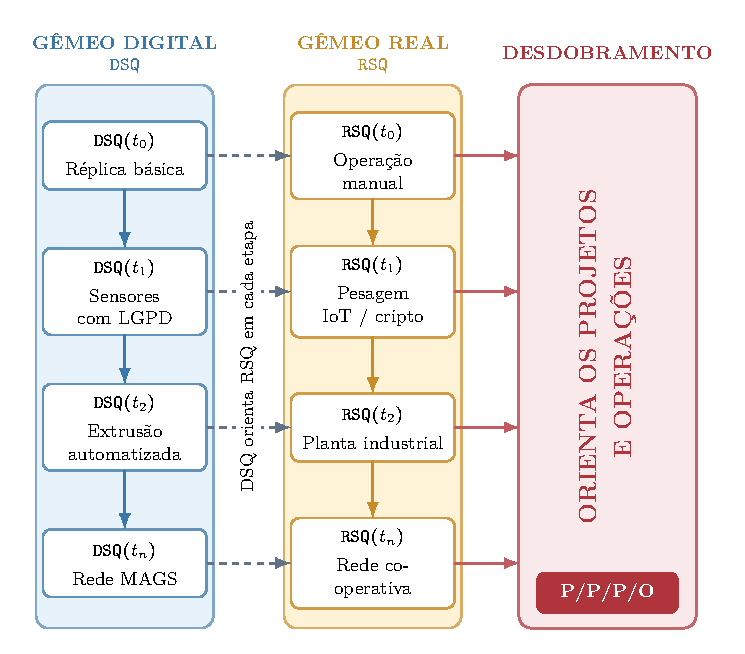
\includegraphics[width=22cm]{out/cadeia1v4.pdf}
\caption{Cadeia de Configurações e Alinhamento $DSQ \rightarrow RSQ$.}
\end{figure}

\vspace{0.3cm}
\LHead{6. Conclusões}

A proposta de extensão \texttt{GPH.SIPA} ao PMBOK 8, associada ao paradigma \emph{Digital Twin-First}, permite estruturar uma proposta de evolução tecnológica para cooperativas de reciclagem. A incorporação de requisitos de privacidade desde a concepção do Gêmeo Digital pode contribuir para a proteção dos dados pessoais dos cooperados e para a melhoria dos processos de governança e gestão.

\end{textblock}

\end{document}
